\documentclass{standalone}
\usepackage{tikz}
\usetikzlibrary{patterns}
\usetikzlibrary{positioning}
\usetikzlibrary{patterns, positioning}
\usetikzlibrary{shapes.misc}
\usepackage[outline]{contour}
\contourlength{1.5pt} 
\usetikzlibrary{calc}
        \usepackage{relsize}
        \tikzset{fontscale/.style = {font=\relsize{#1}}}

\begin{document}
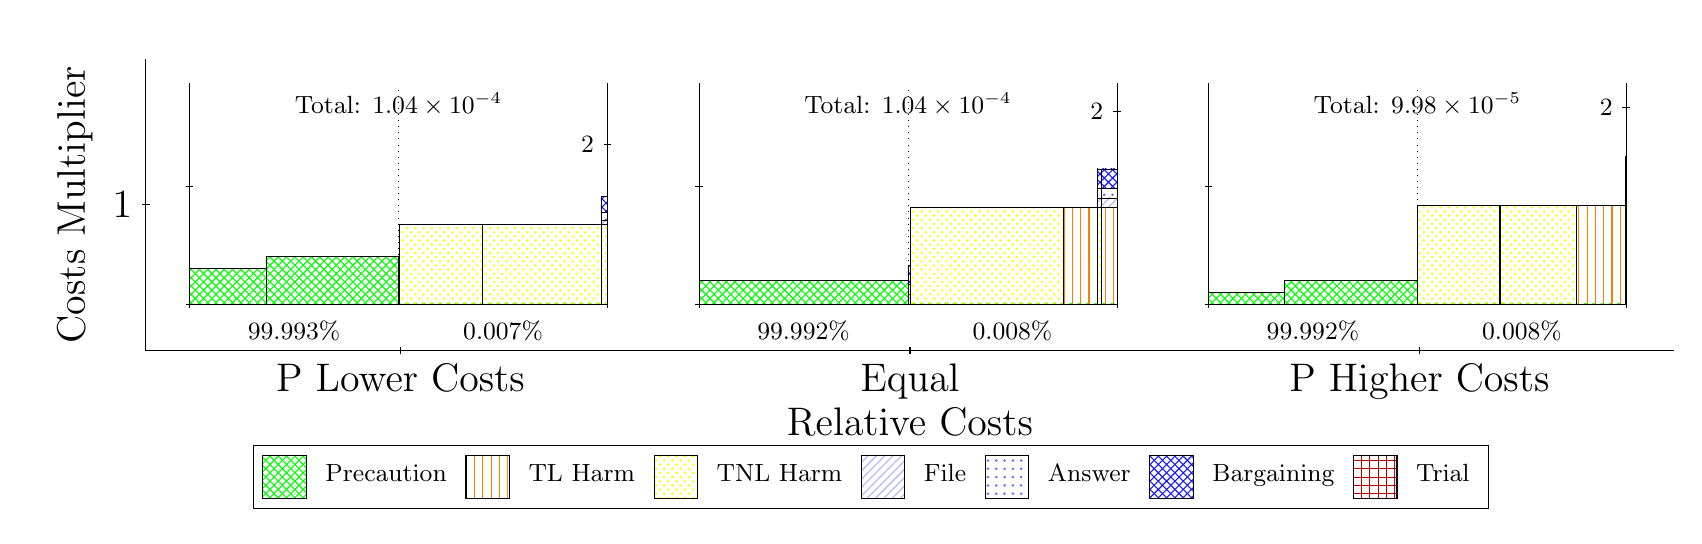
\begin{tikzpicture}
\clip(-0.5,-1.1) rectangle +(20.91,6.2);
\draw[black] (1,1) -- (1,4.7);
\node[rotate=90, fontscale=2, anchor=center] at (0.1, 2.85) {Costs Multiplier};
\draw[black] (0.95,2.85) -- (1.05,2.85);
\node[fontscale=2, anchor=east] at (0.95, 2.85) {1};

\draw[black] (1,1) -- (20.41,1);
\node[fontscale=2, anchor=center] at (10.705, 0.1) {Relative Costs};
\draw[black] (4.235,0.95) -- (4.235,1.05);
\node[fontscale=2, anchor=north] at (4.235, 0.95) {P Lower Costs};
\draw[black] (10.705,0.95) -- (10.705,1.05);
\node[fontscale=2, anchor=north] at (10.705, 0.95) {Equal};
\draw[black] (17.175,0.95) -- (17.175,1.05);
\node[fontscale=2, anchor=north] at (17.175, 0.95) {P Higher Costs};


\draw[pattern=crosshatch, pattern color=green,draw=black,very thin] (1.5556,1.592) rectangle (2.5248,2.042);
\draw[pattern=crosshatch, pattern color=green,draw=black,very thin] (2.5248,1.592) rectangle (4.21,2.192);
\draw[pattern=crosshatch, pattern color=green,draw=black,very thin] (4.21,1.592) rectangle (4.2213,1.592);
\draw[pattern=north east lines, pattern color=blue!30,draw=black,very thin] (4.21,1.592) rectangle (4.2213,1.6426);
\draw[pattern=dots,  pattern color=blue!60,draw=black,very thin] (4.21,1.6426) rectangle (4.2213,1.7439);
\draw[pattern=crosshatch,      pattern color=blue!90,draw=black,very thin] (4.21,1.7439) rectangle (4.2213,1.9463);
\draw[pattern=crosshatch, pattern color=green,draw=black,very thin] (4.2213,1.592) rectangle (5.2711,1.592);
\draw[pattern=crosshatch dots, pattern color=yellow,draw=black,very thin] (4.2213,1.592) rectangle (5.2711,2.6043);
\draw[pattern=crosshatch, pattern color=green,draw=black,very thin] (5.2711,1.592) rectangle (6.7799,1.592);
\draw[pattern=crosshatch dots, pattern color=yellow,draw=black,very thin] (5.2711,1.592) rectangle (6.7799,2.6043);
\draw[pattern=crosshatch, pattern color=green,draw=black,very thin] (6.7799,1.592) rectangle (6.8605,1.592);
\draw[pattern=crosshatch dots, pattern color=yellow,draw=black,very thin] (6.7799,1.592) rectangle (6.8605,2.6043);
\draw[pattern=north east lines, pattern color=blue!30,draw=black,very thin] (6.7799,2.6043) rectangle (6.8605,2.6549);
\draw[pattern=dots,  pattern color=blue!60,draw=black,very thin] (6.7799,2.6549) rectangle (6.8605,2.7561);
\draw[pattern=crosshatch,      pattern color=blue!90,draw=black,very thin] (6.7799,2.7561) rectangle (6.8605,2.9586);
\draw[pattern=crosshatch, pattern color=green,draw=black,very thin] (6.8605,1.592) rectangle (6.8614,1.592);
\draw[pattern=vertical lines, pattern color=orange,draw=black,very thin] (6.8605,1.592) rectangle (6.8614,2.6043);
\draw[pattern=north east lines, pattern color=blue!30,draw=black,very thin] (6.8605,2.6043) rectangle (6.8614,2.6549);
\draw[pattern=dots,  pattern color=blue!60,draw=black,very thin] (6.8605,2.6549) rectangle (6.8614,2.7561);
\draw[pattern=crosshatch,      pattern color=blue!90,draw=black,very thin] (6.8605,2.7561) rectangle (6.8614,2.9586);
\draw[pattern=crosshatch, pattern color=green,draw=black,very thin] (6.8614,1.592) rectangle (6.8644,1.592);
\draw[pattern=crosshatch dots, pattern color=yellow,draw=black,very thin] (6.8614,1.592) rectangle (6.8644,2.6043);
\draw[pattern=north east lines, pattern color=blue!30,draw=black,very thin] (6.8614,2.6043) rectangle (6.8644,2.6549);
\draw[pattern=dots,  pattern color=blue!60,draw=black,very thin] (6.8614,2.6549) rectangle (6.8644,2.7561);
\draw[pattern=crosshatch,      pattern color=blue!90,draw=black,very thin] (6.8614,2.7561) rectangle (6.8644,2.9586);
\draw[pattern=grid,            pattern color=red!70!black,draw=black,very thin] (6.8614,2.9586) rectangle (6.8644,3.1104);
\node[font=\small,text=black,anchor=north] at (4.21, 4.4) {Total: $1.04\times 10^{-4}$};
\draw[black,very thin] (1.5556,1.592) -- (1.5556,4.4);
\draw[black,very thin] (1.5056,1.592) -- (1.6056,1.592);
\node[font=\small,text=black, anchor=west] at (1.5056, 1.592) {};
\draw[black,very thin] (1.5056,3.092) -- (1.6056,3.092);
\node[font=\small,text=black, anchor=west] at (1.5056, 3.092) {};

\draw[black,dotted,very thin] (4.21,1.6762) -- (4.21,4.3158);
\draw[black,very thin] (6.8644,1.592) -- (6.8644,4.4);
\draw[black,very thin] (6.8144,3.6165) -- (6.9144,3.6165);
\node[font=\small,text=black, anchor=east] at (6.8144, 3.6165) {\contour{white}{2}};

\draw[black,very thin] (1.5556,1.592) -- (6.8644,1.592);
\draw[black,very thin] (1.5556,1.542) -- (1.5556,1.642);
\node[font=\small,text=black, anchor=north] at (1.5556, 1.542) {};
\draw[black,very thin] (6.8644,1.542) -- (6.8644,1.642);
\node[font=\small,text=black, anchor=north] at (6.8644, 1.542) {};

\node[font=\small,text=black,anchor=south] at (2.8828, 0.992) {99.993\%};
\node[font=\small,text=black,anchor=south] at (5.5372, 0.992) {0.007\%};

\draw[pattern=crosshatch, pattern color=green,draw=black,very thin] (8.0256,1.592) rectangle (10.68,1.892);
\draw[pattern=crosshatch, pattern color=green,draw=black,very thin] (10.68,1.592) rectangle (10.713,1.592);
\draw[pattern=north east lines, pattern color=blue!30,draw=black,very thin] (10.68,1.592) rectangle (10.713,1.7144);
\draw[pattern=dots,  pattern color=blue!60,draw=black,very thin] (10.68,1.7144) rectangle (10.713,1.8369);
\draw[pattern=crosshatch,      pattern color=blue!90,draw=black,very thin] (10.68,1.8369) rectangle (10.713,2.0817);
\draw[pattern=crosshatch, pattern color=green,draw=black,very thin] (10.713,1.592) rectangle (12.648,1.592);
\draw[pattern=crosshatch dots, pattern color=yellow,draw=black,very thin] (10.713,1.592) rectangle (12.648,2.8162);
\draw[pattern=crosshatch, pattern color=green,draw=black,very thin] (12.648,1.592) rectangle (13.083,1.592);
\draw[pattern=vertical lines, pattern color=orange,draw=black,very thin] (12.648,1.592) rectangle (13.083,2.8162);
\draw[pattern=crosshatch, pattern color=green,draw=black,very thin] (13.083,1.592) rectangle (13.131,1.592);
\draw[pattern=crosshatch dots, pattern color=yellow,draw=black,very thin] (13.083,1.592) rectangle (13.131,2.8162);
\draw[pattern=north east lines, pattern color=blue!30,draw=black,very thin] (13.083,2.8162) rectangle (13.131,2.9386);
\draw[pattern=dots,  pattern color=blue!60,draw=black,very thin] (13.083,2.9386) rectangle (13.131,3.061);
\draw[pattern=crosshatch,      pattern color=blue!90,draw=black,very thin] (13.083,3.061) rectangle (13.131,3.3059);
\draw[pattern=crosshatch, pattern color=green,draw=black,very thin] (13.131,1.592) rectangle (13.334,1.592);
\draw[pattern=vertical lines, pattern color=orange,draw=black,very thin] (13.131,1.592) rectangle (13.334,2.8162);
\draw[pattern=north east lines, pattern color=blue!30,draw=black,very thin] (13.131,2.8162) rectangle (13.334,2.9386);
\draw[pattern=dots,  pattern color=blue!60,draw=black,very thin] (13.131,2.9386) rectangle (13.334,3.061);
\draw[pattern=crosshatch,      pattern color=blue!90,draw=black,very thin] (13.131,3.061) rectangle (13.334,3.3059);
\draw[pattern=crosshatch, pattern color=green,draw=black,very thin] (13.334,1.592) rectangle (13.334,1.592);
\draw[pattern=crosshatch dots, pattern color=yellow,draw=black,very thin] (13.334,1.592) rectangle (13.334,2.8162);
\draw[pattern=north east lines, pattern color=blue!30,draw=black,very thin] (13.334,2.8162) rectangle (13.334,2.9386);
\draw[pattern=dots,  pattern color=blue!60,draw=black,very thin] (13.334,2.9386) rectangle (13.334,3.061);
\draw[pattern=crosshatch,      pattern color=blue!90,draw=black,very thin] (13.334,3.061) rectangle (13.334,3.3059);
\draw[pattern=grid,            pattern color=red!70!black,draw=black,very thin] (13.334,3.3059) rectangle (13.334,3.5507);
\node[font=\small,text=black,anchor=north] at (10.68, 4.4) {Total: $1.04\times 10^{-4}$};
\draw[black,very thin] (8.0256,1.592) -- (8.0256,4.4);
\draw[black,very thin] (7.9756,1.592) -- (8.0756,1.592);
\node[font=\small,text=black, anchor=west] at (7.9756, 1.592) {};
\draw[black,very thin] (7.9756,3.0919) -- (8.0756,3.0919);
\node[font=\small,text=black, anchor=west] at (7.9756, 3.0919) {};

\draw[black,dotted,very thin] (10.68,1.6762) -- (10.68,4.3158);
\draw[black,very thin] (13.334,1.592) -- (13.334,4.4);
\draw[black,very thin] (13.284,4.0403) -- (13.384,4.0403);
\node[font=\small,text=black, anchor=east] at (13.284, 4.0403) {\contour{white}{2}};

\draw[black,very thin] (8.0256,1.592) -- (13.334,1.592);
\draw[black,very thin] (8.0256,1.542) -- (8.0256,1.642);
\node[font=\small,text=black, anchor=north] at (8.0256, 1.542) {};
\draw[black,very thin] (13.334,1.542) -- (13.334,1.642);
\node[font=\small,text=black, anchor=north] at (13.334, 1.542) {};

\node[font=\small,text=black,anchor=south] at (9.3528, 0.992) {99.992\%};
\node[font=\small,text=black,anchor=south] at (12.007, 0.992) {0.008\%};

\draw[pattern=crosshatch, pattern color=green,draw=black,very thin] (14.496,1.592) rectangle (15.465,1.742);
\draw[pattern=crosshatch, pattern color=green,draw=black,very thin] (15.465,1.592) rectangle (17.15,1.892);
\draw[pattern=crosshatch, pattern color=green,draw=black,very thin] (17.15,1.592) rectangle (17.152,1.592);
\draw[pattern=north east lines, pattern color=blue!30,draw=black,very thin] (17.15,1.592) rectangle (17.152,1.8416);
\draw[pattern=dots,  pattern color=blue!60,draw=black,very thin] (17.15,1.8416) rectangle (17.152,1.9664);
\draw[pattern=crosshatch,      pattern color=blue!90,draw=black,very thin] (17.15,1.9664) rectangle (17.152,2.216);
\draw[pattern=crosshatch, pattern color=green,draw=black,very thin] (17.152,1.592) rectangle (18.189,1.592);
\draw[pattern=crosshatch dots, pattern color=yellow,draw=black,very thin] (17.152,1.592) rectangle (18.189,2.84);
\draw[pattern=crosshatch, pattern color=green,draw=black,very thin] (18.189,1.592) rectangle (18.206,1.592);
\draw[pattern=vertical lines, pattern color=orange,draw=black,very thin] (18.189,1.592) rectangle (18.206,2.84);
\draw[pattern=crosshatch, pattern color=green,draw=black,very thin] (18.206,1.592) rectangle (19.165,1.592);
\draw[pattern=crosshatch dots, pattern color=yellow,draw=black,very thin] (18.206,1.592) rectangle (19.165,2.84);
\draw[pattern=crosshatch, pattern color=green,draw=black,very thin] (19.165,1.592) rectangle (19.786,1.592);
\draw[pattern=vertical lines, pattern color=orange,draw=black,very thin] (19.165,1.592) rectangle (19.786,2.84);
\draw[pattern=crosshatch, pattern color=green,draw=black,very thin] (19.786,1.592) rectangle (19.795,1.592);
\draw[pattern=crosshatch dots, pattern color=yellow,draw=black,very thin] (19.786,1.592) rectangle (19.795,2.84);
\draw[pattern=north east lines, pattern color=blue!30,draw=black,very thin] (19.786,2.84) rectangle (19.795,3.0896);
\draw[pattern=dots,  pattern color=blue!60,draw=black,very thin] (19.786,3.0896) rectangle (19.795,3.2144);
\draw[pattern=crosshatch,      pattern color=blue!90,draw=black,very thin] (19.786,3.2144) rectangle (19.795,3.464);
\draw[pattern=crosshatch, pattern color=green,draw=black,very thin] (19.795,1.592) rectangle (19.801,1.592);
\draw[pattern=vertical lines, pattern color=orange,draw=black,very thin] (19.795,1.592) rectangle (19.801,2.84);
\draw[pattern=north east lines, pattern color=blue!30,draw=black,very thin] (19.795,2.84) rectangle (19.801,3.0896);
\draw[pattern=dots,  pattern color=blue!60,draw=black,very thin] (19.795,3.0896) rectangle (19.801,3.2144);
\draw[pattern=crosshatch,      pattern color=blue!90,draw=black,very thin] (19.795,3.2144) rectangle (19.801,3.464);
\draw[pattern=crosshatch, pattern color=green,draw=black,very thin] (19.801,1.592) rectangle (19.803,1.592);
\draw[pattern=crosshatch dots, pattern color=yellow,draw=black,very thin] (19.801,1.592) rectangle (19.803,2.84);
\draw[pattern=north east lines, pattern color=blue!30,draw=black,very thin] (19.801,2.84) rectangle (19.803,3.0896);
\draw[pattern=dots,  pattern color=blue!60,draw=black,very thin] (19.801,3.0896) rectangle (19.803,3.2144);
\draw[pattern=crosshatch,      pattern color=blue!90,draw=black,very thin] (19.801,3.2144) rectangle (19.803,3.464);
\draw[pattern=grid,            pattern color=red!70!black,draw=black,very thin] (19.801,3.464) rectangle (19.803,3.8384);
\draw[pattern=crosshatch, pattern color=green,draw=black,very thin] (19.803,1.592) rectangle (19.804,1.592);
\draw[pattern=vertical lines, pattern color=orange,draw=black,very thin] (19.803,1.592) rectangle (19.804,2.84);
\draw[pattern=north east lines, pattern color=blue!30,draw=black,very thin] (19.803,2.84) rectangle (19.804,3.0896);
\draw[pattern=dots,  pattern color=blue!60,draw=black,very thin] (19.803,3.0896) rectangle (19.804,3.2144);
\draw[pattern=crosshatch,      pattern color=blue!90,draw=black,very thin] (19.803,3.2144) rectangle (19.804,3.464);
\draw[pattern=grid,            pattern color=red!70!black,draw=black,very thin] (19.803,3.464) rectangle (19.804,3.8384);
\node[font=\small,text=black,anchor=north] at (17.15, 4.4) {Total: $9.98\times 10^{-5}$};
\draw[black,very thin] (14.496,1.592) -- (14.496,4.4);
\draw[black,very thin] (14.446,1.592) -- (14.546,1.592);
\node[font=\small,text=black, anchor=west] at (14.446, 1.592) {};
\draw[black,very thin] (14.446,3.0919) -- (14.546,3.0919);
\node[font=\small,text=black, anchor=west] at (14.446, 3.0919) {};

\draw[black,dotted,very thin] (17.15,1.6762) -- (17.15,4.3158);
\draw[black,very thin] (19.804,1.592) -- (19.804,4.4);
\draw[black,very thin] (19.754,4.088) -- (19.854,4.088);
\node[font=\small,text=black, anchor=east] at (19.754, 4.088) {\contour{white}{2}};

\draw[black,very thin] (14.496,1.592) -- (19.804,1.592);
\draw[black,very thin] (14.496,1.542) -- (14.496,1.642);
\node[font=\small,text=black, anchor=north] at (14.496, 1.542) {};
\draw[black,very thin] (19.804,1.542) -- (19.804,1.642);
\node[font=\small,text=black, anchor=north] at (19.804, 1.542) {};

\node[font=\small,text=black,anchor=south] at (15.823, 0.992) {99.992\%};
\node[font=\small,text=black,anchor=south] at (18.477, 0.992) {0.008\%};

\coordinate (LegendAnchor) at (10.205000000000002,0);
\begin{scope}[align=center]
\matrix[scale=0.6,draw=black,below=0.2cm of LegendAnchor,nodes={draw},column sep=0.12cm]{
\node[rectangle,draw,minimum width=0.55cm,minimum height=0.55cm,pattern=crosshatch, pattern color=green]{}; &
        \node[draw=none,font=\small]{Precaution}; &
\node[rectangle,draw,minimum width=0.55cm,minimum height=0.55cm,pattern=vertical lines, pattern color=orange]{}; &
        \node[draw=none,font=\small]{TL Harm}; &
\node[rectangle,draw,minimum width=0.55cm,minimum height=0.55cm,pattern=crosshatch dots, pattern color=yellow]{}; &
        \node[draw=none,font=\small]{TNL Harm}; &
\node[rectangle,draw,minimum width=0.55cm,minimum height=0.55cm,pattern=north east lines, pattern color=blue!30]{}; &
        \node[draw=none,font=\small]{File}; &
\node[rectangle,draw,minimum width=0.55cm,minimum height=0.55cm,pattern=dots, pattern color=blue!60]{}; &
        \node[draw=none,font=\small]{Answer}; &
\node[rectangle,draw,minimum width=0.55cm,minimum height=0.55cm,pattern=crosshatch, pattern color=blue!90]{}; &
        \node[draw=none,font=\small]{Bargaining}; &
\node[rectangle,draw,minimum width=0.55cm,minimum height=0.55cm,pattern=grid, pattern color=red!70!black]{}; &
        \node[draw=none,font=\small]{Trial}; \\
};\end{scope}

\end{tikzpicture}
\end{document}